\subsection{Network traffic}
\label{sec:networktraffic}
\paragraph{Programmable end node}
The software for the \textit{programmable end nodes} implementing the required functions is decoupled from the physical node it is deployed on. From a programmers point of view the software is split up un several logical nodes. Each node is responsible for implementing a certain related set of functions, examples of logical nodes are: the \textit{Braking System Manager} or the \textit{Lighting Manager}. The logical nodes consist of one or more runnables, the runnable is the smallest software component that is subject to scheduling by the RTOS. This allows to split a logical node in several runnables which can be scheduled independently or deployed on different physical nodes. Runnables communicate with each other through signals, a signal represents a sample of some system state variable. These system state variables can represent a physical value or an abstract value. For example as displayed in Figure~\ref{fig:logical}, \textit{brake pedal applied} could be a signal generated by a runnable of the \textit{Braking System Manager}, describing whether the brake pedal is being pressed by the driver. A \textit{Lighting Manager} runnable could consume the \textit{brake pedal applied} signal to determine whether the brake lights should be lit. A signal is produced by a single runnable, but can be consumed by multiple runnables. For each logical node a set of deployment files describe which runnables exist, which signals are consumed and produced by each runnable, at what rate the runnables are scheduled and on which \textit{programmable end nodes} they are deployed.

\begin{figure}[htbp]
    \centering
    \resizebox{0.95\textwidth}{!}{%
        \tikzfig{logical_example}
    }
 \caption{Example of two logical components consisting of several runnables communicating through signals}
\label{fig:logical}
\end{figure}

The deployment files are used when building binaries for the \textit{programmable end nodes} to automatically generate code to bridge the required signals between the runnables. First let's consider a pair of runnables consuming/producing the same signal that are deployed on the same \textit{programmable end node}. So one runnable generates a signal while the other is a consumer of that signal. Because the runnables are deployed on the same \textit{programmable end nodes} there is no network traffic necessary. In this case the signal can be thought of as being implemented as a global variable residing in the \textit{programmable end nodes} memory which can be accessed in a thread-safe way by both runnables.

If the producing and consuming runnables are deployed on different \textit{programmable end nodes} which are directly connected to each other e.g, the Vehicle Control Unit and the Central Gateway, the signal has to be transmitted on the network connecting them. In this case the signal is transmitted to the receiving node over CAN at a fixed rate. For efficiency reasons signals that have the same \textit{programmable end node} as destination are packed in the same CAN message. See Figure~\ref{fig:deployment} for an example deployment of two logical nodes, a \textit{Vehicle Power Controller} consisting of two runnables, and the \textit{Exterior Lighting} logical consisting of a single runnable. And two signals \textit{active\_gear} and \textit{power\_mode} that are produced and consumed by the runnables.

\begin{figure}[htbp]
    \centering
    \resizebox{\textwidth}{!}{%
        \tikzfig{deployment_example}
    }
 \caption{Example of two logical components consisting of several runnables communicating through signals}
\label{fig:deployment}
\end{figure}

The last case is when a producing and consuming runnable are deployed on different \textit{programmable end nodes} which are not directly connected to each other e.g, the Vehicle Control Unit and Safety Control Unit. In this case the message has to be bridged across two networks by the Central Gateway. For modelling purposes one can think of having two runnables in the Central Gateway responsible for bridging the data from node A to B. The first being the \textit{gateway\_receive} runnable, which consumes signals from node A. The second being the \textit{gateway\_transmit} runnable, which produces signals for the runnables running on \textit{programmable end node} B, forwarding the consumed signal from the \textit{gateway\_receive} runnable.

Because signals can be consumed by multiple runnables, combinations of the cases mentioned above are possible for a single signal. For example a signal can be consumed by a runnable deployed on the same \textit{programmable end node} and by a runnable on a node without direct CAN connection, requiring bridging by the Central Gateway.

Because the deployment can change as development progresses but also because a deployment is specific to a vehicle type we want to create a description of the data flow on the logical level. This description can be used as an input for generating several deployments whose performance can be evaluated using simulation. The data flow description is specific for a vehicle as it is influenced by the chosen architecture and the feature set. It can serve as a benchmark for a type of vehicle with a known feature set. The data flow description can be adapted to match vehicles with different architectures and feature sets. 

From the deployment files we can generate an interface overview of the \textit{programmable end node} software i.e, a list detailing the source runnable of a signal and which runnables consume that signal together with several other signal attributes such as the data type (integer, enumerate, etc.). This gives us a part of the logical architecture data flow. As described earlier the runnables executing on the \textit{programmable end nodes} generate network traffic when signals are shared between runnables on separate nodes. The deployment files contain the mapping of runnable to \textit{programmable end node}, together with the logical data flow it is possible to generate an interface overview detailing the source and destination in the physical architecture for each signal. A script has been created to generate such interface overviews both in tabular (machine readable) form, for further processing by to be created software as in graphical form to aid in debugging issues in the vehicle. Table~\ref{tab:interface_overview} shows the tabular output of the script for two signals in the Lightyear 0, the \textit{active\_gear} signal is produced by the \textit{Vehicle Power Controler} logical component in the primary core of the \textit{Safety Control Unit} ECU, it is consumed by three other logicals executing in the \textit{Safety Control Unit} primary core and by four logicals executing in two different \textit{programmable end nodes}. Figure~\ref{fig:interface_overview} displays the same information in a directed graph. The circular nodes represent the signal while the rectangular nodes represent the runnable consuming/producing the signal. An edge originating in the signal node and ending in a runnable node represents that the signal is consumed by the destination runnable. An edge originating in a runnable node and ending in the signal node represents that the runnable produces the signal.

\begin{table}[htbp]
    \centering
    \resizebox{\textwidth}{!}{%
    \begin{tabular}{@{}llllll@{}}
    \toprule
    signal name  & source physical  & source logical           & destination physical   & destination logical         & data type        \\ \midrule
    active\_gear & scu\_primary     & Vehicle Power Controller & scu\_primary           & Braking System Manager      & int16\_t         \\
    power\_mode  & central\_gateway & VPC Gateway              & scu\_primary           & Vehicle Power Controller    & i\_psm\_state\_t \\
    power\_mode  & central\_gateway & VPC Gateway              & scu\_primary           & Energy Storage Controller   & i\_psm\_state\_t \\
    active\_gear & scu\_primary     & Vehicle Power Controller & scu\_primary           & Gear Selector Manager       & int16\_t         \\
    active\_gear & scu\_primary     & Vehicle Power Controller & scu\_primary           & Safety Supervisor Core      & int16\_t         \\
    power\_mode  & central\_gateway & VPC Gateway              & scu\_primary           & Safety Supervisor Core      & i\_psm\_state\_t \\
    active\_gear & scu\_primary     & Vehicle Power Controller & central\_gateway       & Authentication Manager      & int16\_t         \\
    active\_gear & scu\_primary     & Vehicle Power Controller & central\_gateway       & Media ECU Interface Manager & int16\_t         \\
    active\_gear & scu\_primary     & Vehicle Power Controller & central\_gateway       & Lighting Manager            & int16\_t         \\
    active\_gear & scu\_primary     & Vehicle Power Controller & vehicle\_control\_unit & Driver Controls Manager     & int16\_t         \\
    power\_mode  & central\_gateway & VPC Gateway              & vehicle\_control\_unit & Solar Controller            & i\_psm\_state\_t \\
    power\_mode  & central\_gateway & VPC Gateway              & vehicle\_control\_unit & VPC vcu                     & i\_psm\_state\_t \\ \bottomrule
    \end{tabular}%
    }
    \caption{Interface overview for \textit{power\_mode} and \textit{active\_gear} signals}
    \label{tab:interface_overview}
    \end{table}

\begin{figure}[htbp]
    \centering
    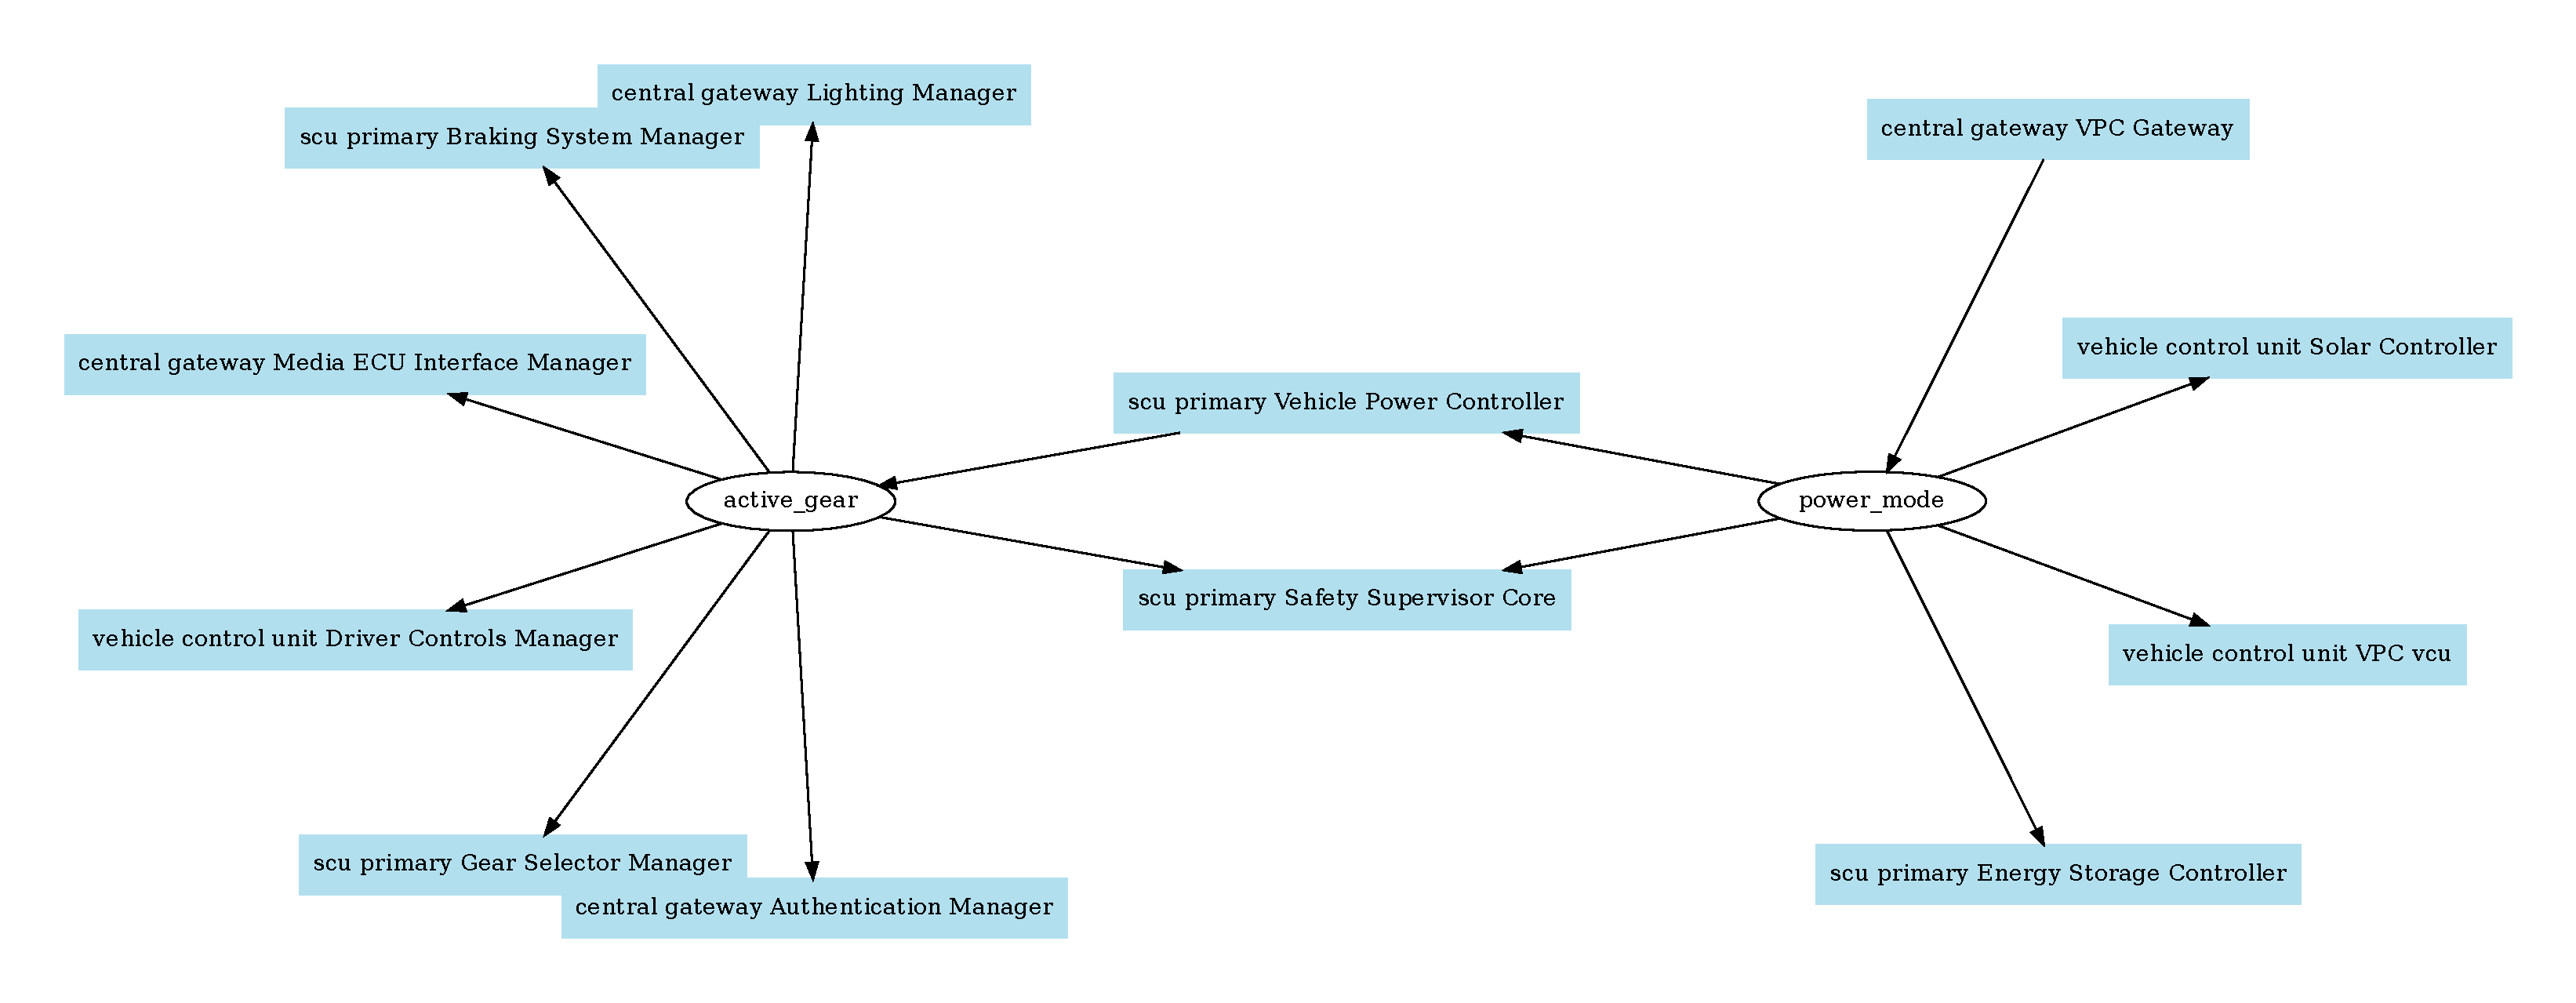
\includegraphics[width=\textwidth]{images/interface_overview.pdf}
    \caption{Interface overview for two signals in graphical form}
    \label{fig:interface_overview}
\end{figure}

\paragraph{Parametrizable end nodes}
The network traffic to and from \textit{parametrizable end nodes} is described in special deployment files called DBC files for CAN networks and LDF files for LIN networks. These are industry standards describing the messages that can be found on a network. For each message the content is described in terms of signals and how the raw bytes transmitted on the network map to a signal value. For example a signal \textit{brake pedal position} describing a numerical value has a certain data type (single precision floating point, 16-bit signed integer, 32-bit unsigned integer), but the numerical value can be also scaled and offset to represent the real value. The DBC and LDF standards describe how a set of received bytes can be reinterpreted as the original signal and how a measured value must be transformed in a set of bytes to transmit. 

In order to get the data flow to and from \textit{parametrizable end nodes} the LDF and DBC files are necessary as they describe which signals are communicated. Unfortunately these files do not always describe the source and destination of a signal, nor do they accurately describe the transmission rate, nor is it known which runnable from the \textit{programmable end nodes} consumes/produces the signal. This information is not available in a central and easily machine-readable format. A possible solution for partially retrieving this information is through static analysis of the \textit{programmable end node} software. The reception and transmission of the signals using the CAN and LIN busses happens by using a specific set of interfaces provided by the RTOS. By analysing call graphs of these interfaces the missing information could be retrieved. Some inaccuracies in the exact transmission rate of the signals might be introduced, but that is an acceptable risk given that we are using the data flow description as an input for simulating and evaluating various network configurations. A second solution would be to assume that each node on the bus consumes the transmitted data at exactly the rate at which it is transmitted. This would solve the lack of source and destination information but still misses the transmission rate. Additionally, it would introduce inaccuracies that could make the data flow description too pessimistic.

\paragraph{Aperiodic and non-real time data}
The description of dataflow by the various nodes so far serves as input/output of the various control applications in the vehicle e.g, cruise control or battery management, this type of traffic is (mostly) periodic and has a defined transmission rate. Data that is unrelated to the control systems is served on the same networks. For example applications such as software updates, remote diagnostics, logging of crucial signals all generate data that requires bandwidth on the network to reach the appropriate destination. To accommodate the complex requirements of these applications a transport layer is used to allow transmitting data packets with a data size that is larger than the maximum data size of a CAN frame. The chosen protocol is ISO~15765, known as ISO-TP, which acts as the network and transport layer in the OSI model.
\todo{Check which aperiodic data is generated by parametrizable/programmable end nodes}

The Telematics Control Unit (TCU) regularly checks if software updates are available, when an update is initiated the TCU transmits the update using ISO-TP to the end node that is updated. Because the TCU only has a direct CAN connection with the Central Gateway the update stream must be bridged by the Central Gateway to the correct CAN bus. When the to be updated end node has no direct connection with the Central Gateway, such as the inverters (Table~\ref{tab:networks}), the stream must be bridged again in this example by the Safety Control Unit. Similarly, logging of crucial signals occurs in an online database. The data is collected by the \textit{programmable end nodes} and transmitted to the TCU using ISO-TP. 

When a vehicle has to be serviced a technician can connect to the diagnostics port and run diagnostics using the industry standard ISO~14229 - Unified Diagnostic Services (UDS). UDS is a communication protocol specifically designed for diagnostics in vehicles. It allows technicians to read error codes of all the nodes in the network, perform tests and configure certain parameters. UDS uses ISO-TP as the transport layer, as the diagnostics port is connected to the Central Gateway bridging of the UDS messages occurs similarly to the software update stream when an end node is not directly connected to the Central Gateway.

\todo{Describe ethernet traffic}